\documentclass[10pt,a4paper]{article}
\usepackage[latin1]{inputenc}
\usepackage{amsmath}
\usepackage{amsfonts}
\usepackage{amssymb}
\usepackage{graphicx}
\usepackage{listings}
\usepackage[nottoc]{tocbibind}
\author{Baptiste Pauget}
\title{M1 Internship : Compiling Whiley to FPGAs}

\begin{document}
\maketitle
\section*{Introduction}
\tableofcontents

\section{FPGA compilation}

\subsection{FPGA : a specific hardware}

\subsubsection{Usage}

A Field Programmable Gate Array (FPGAs) is an integrated circuit that can be configure by the user.
It tries to gather the power of Application Specific Integrated Circuits (ASICs) with the flexibility of general computation devices (CPUs), by giving a way to reconfigure hardware without physical operations.

FPGAs enable a faster and less energy consuming computation for specific applications, and they are thus used mainly in :
\begin{itemize}
	\item \textbf{Prototyping ASICs} : ASICs are still faster than FPGAs but their development requires one to create new physical circuits to test them, thus FPGAs can make the process easier and cheaper.
	\item \textbf{Computation helpers} : The performances specific applications (images processing, ...) can be enhanced with hardware compiled function (FFT), and FPGAs are an easy way to do so.
	\item \textbf{Highly parallel applications} : because of their high parallelism potential, FPGAs are useful in applications processing lots of data simultaneously, like network interfaces (where large bandwidth is needed).
\end{itemize}

To use the device, a configuration has to be loaded at each power on (the configuration storage is RAM based and lost when the FPGA is not powered).

\subsubsection{Structural organisation}

FPGAs are organised as a array of interconnected computation cells, with some specific components.

\begin{figure}[h]
	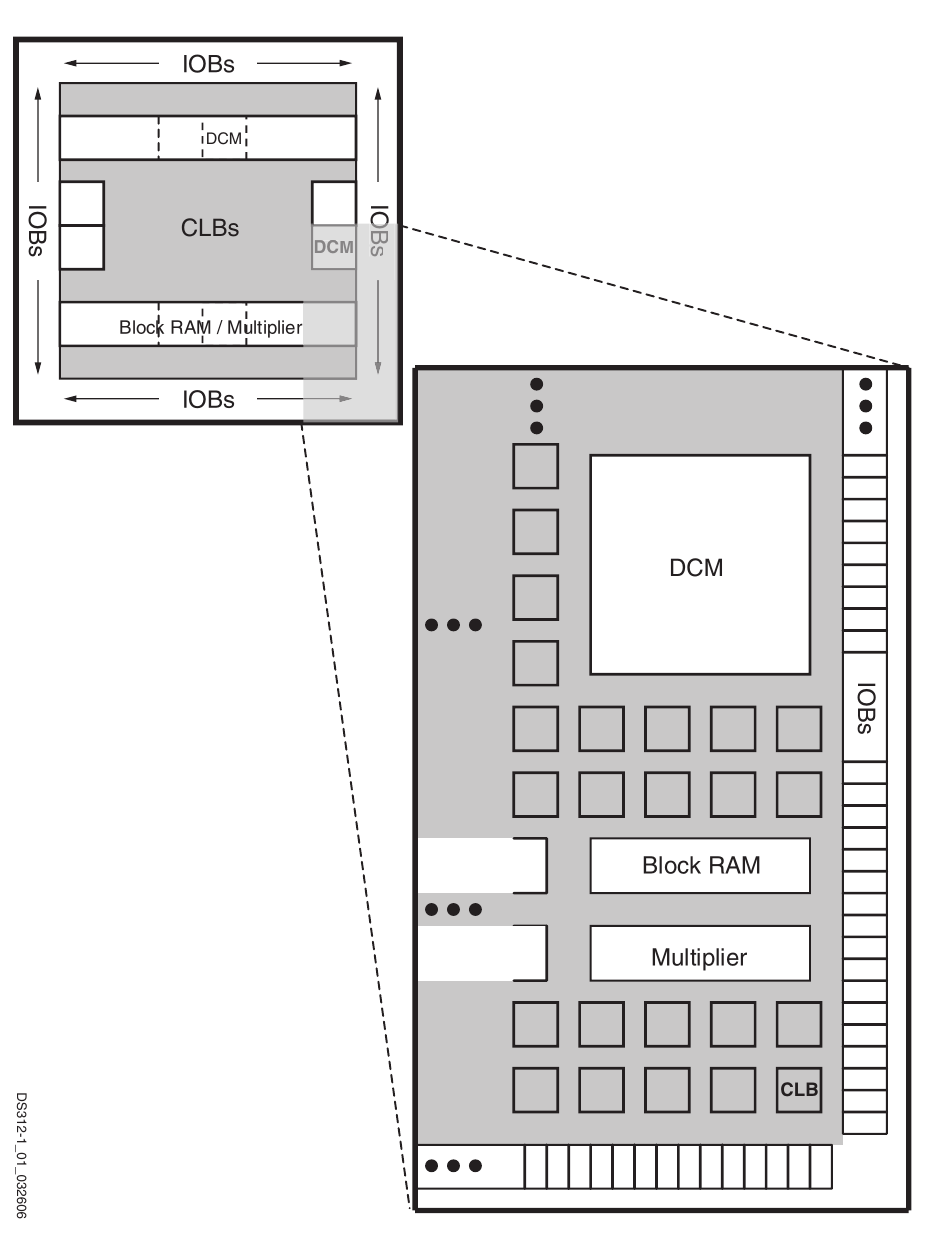
\includegraphics[scale=0.3]{Spartan.png}
	\caption{Spartan-3A Platform Architecture \cite{Spartan}}
\end{figure}

Here are the major architecture components of Xilinx Spartan-3 FPGAs \cite{Spartan}. 
The numbers give the composition of the Spartan XC3S500E FPGA.

\begin{itemize}
	\item \textbf{Configurable Logic Blocks (CLB)} (1,164) : The atomic units of FPGAs.
	They are divided in 4 slices  containing
	\begin{itemize}
		\item \textbf{2 Look-Up Tables} (LUT) : Implementation of logic computation in small LUTs (4 to 1 bits) that enable to compute any boolean function (They are RAM memory based)
		\item \textbf{2 Storage Elements} : Can be used as flip-flops or latches
	\end{itemize}
	\item \textbf{Input/Outputs Blocks} (232) : They provide an interface to the outside, preserving the internal impedances used in the FPGA.
	\item \textbf{RAM Blocks} (20 : 368,640 bits) : These 18Kbits blocks can be used as RAM/ROM, with up to two I/O ports, with several memory organisation. (reading up to 36 bits with each port).
	\item \textbf{Multipliers Blocks} (20) : They avoid an overuse of CLBs for multiplicative operations.
	\item \textbf{Digital Clock Manager Blocks} : They can duplicate, multiply, divide and delay clock signals
	
\end{itemize}

Some additional specific logic provide improved performances for specific operations (carry/arithmetic logic, dedicated multiplexers, ...).

\subsubsection{Introducing time}

The use of time is provided by external clocks. Usual boards that contain FPGAs include several clocks connected with predefined input ports. Using the specific clock manager blocks, the signals can be duplicated and the frequency changed.

\subsubsection{Parallelism and execution model}

All the CLBs are independent and can be updated at the same time. See section \ref{Concurr}
for details about how this parallelism is supported in the FPGA configuration language.

This feature can be used to duplicate circuits and provide calculation on vector of data rather than a single value at a time or it can support the simultaneous computation of independent parts of the process.


\subsection{The Hardware Description Languages - VHDL}

FPGA's configurations were originally design with circuit diagrams (as done for ASIC projects) but are know made using hardware description languages (HDLs). The main ones are Verilog and VHDL.

\subsubsection{Other HDLs : Verilog}


Verilog

\subsubsection{Structure}

The following design units structure VHDL code :

\paragraph{Package/Library}~\\
Organise the different entities in groups.

\paragraph{Entity}~\\
It provides the interface of a wire circuit to be used in other implementations. It declares the typed input and output ports of the component.

\paragraph{Architecture}~\\
It contains the implementation of an entity. Several architectures can be provided for one entity, and some statements enable to choose the one to use. The body of an architecture is made of several concurrent statements.

\subsubsection{Architecture's content}

\paragraph{Concurrent Statements}
~\\ \label{Concurr}
These statements are mutually independent and their order of declaration is meaningless. They are evaluated when an event occurs on a signals they are sensitive to occur. The modification of a signal's value will thus trigger the computation of every statement using this signal at the same time. The major types of concurrent statements are :

\begin{itemize}
	\item \textbf{Signal assignments} (\textless=) that gives a name to the result of a expression for future use
	\item \textbf{Conditional signal assignment} (when/select) that construct a multiplexer
	\item \textbf{Component instantiations} that instantiates an entity interface with internal signal
	\item \textbf{Process statement} that introduces an other level of description ( discussed below).
\end{itemize}


\paragraph{Sequential Statements}
~\\
Process statements introduce behavioural description. It is closer to that is found in a software programming language : when a process statement is evaluated, the sequential statements it contains are computed respecting their order and some higher level abstractions are available :

\begin{itemize}
	\item \textbf{Variables} can be defined and used in a similar way as for a software programming language, holding different values through the process.
	\item \textbf{If statements} introduce disjunctions (contrary to multiplexers, the variables/signals don't need to be defined in each alternative).
\end{itemize}

The synthesizer convert it to a hardware configuration that will behave the way described in the Process statement. This work is quiet long and can produce large configurations.


A major limitation of process lies in the fact components can't be instantiated inside a process.

The processes appears as a black box for the other concurrent statements of the architecture : the update of the modified signals is seen as simultaneous.

Because the concurrent statement is the only one with an explicit sensitivity list, it is used to introduce signals that change only on the modification of other ones (clocks for example). This is the way register-based memory is introduced.

\subsubsection{Registers}

Registers are signals that keep the same value between the events of other signals. They are mainly used with a clock as trigger.

They are inferred by the synthesizer when an incomplete if statements is encounter : if a signal is set in only some branches of the disjunction, a register will be generated.



\begin{lstlisting}[language=VHDL, frame=single, numbers=left, title=Example of register generation]
  Regist: process(clock) is
  begin
    if (rising_edge(clock)) then
      reg <= newValue;
    end if;
  end process Regist;
\end{lstlisting}


Because generated registers is an indirect process, the if statements have to be carefully used to avoid unwanted effects.

\subsection{The compilation process}

The compilation of VHDL code to FPGA configuration file is a complex and time consuming process. It notably differs from software programming language compilation because of the physical constraints required by the targeted device.

\subsubsection{Tools}

Because the resulting files strongly depends on the FPGA features, the compilation of VHDL code to an effective FPGA configuration is provided by the commercial tools of the FPGA vendors.


\subsubsection{Synthesis step}

The major steps of the compilation process are

\begin{itemize}
	\item \textbf{Parsing and type checking} : Verification that the code is well-formed
	\item \textbf{Synthesis} : Production of net-lists.
	\item \textbf{Mapping} : Conversion of the net-lists to LUTs.
	\item \textbf{Place and route} : Positioning the LUTs and specific blocks on the FPGA, regarding the constraints (output pins, clocks), and drawing the connections
	\item \textbf{Time analysis} : Circuit analysis to determine the longest delay (clock)
	\item \textbf{Configuration generation} : Generating a configuration file for the FPGA.
\end{itemize}

\subsubsection{Simulations}

Because of the expensive time cost of the synthesis and the poor debugging aids, simulators provide a way to enhance the development process.

\begin{figure}[h]
	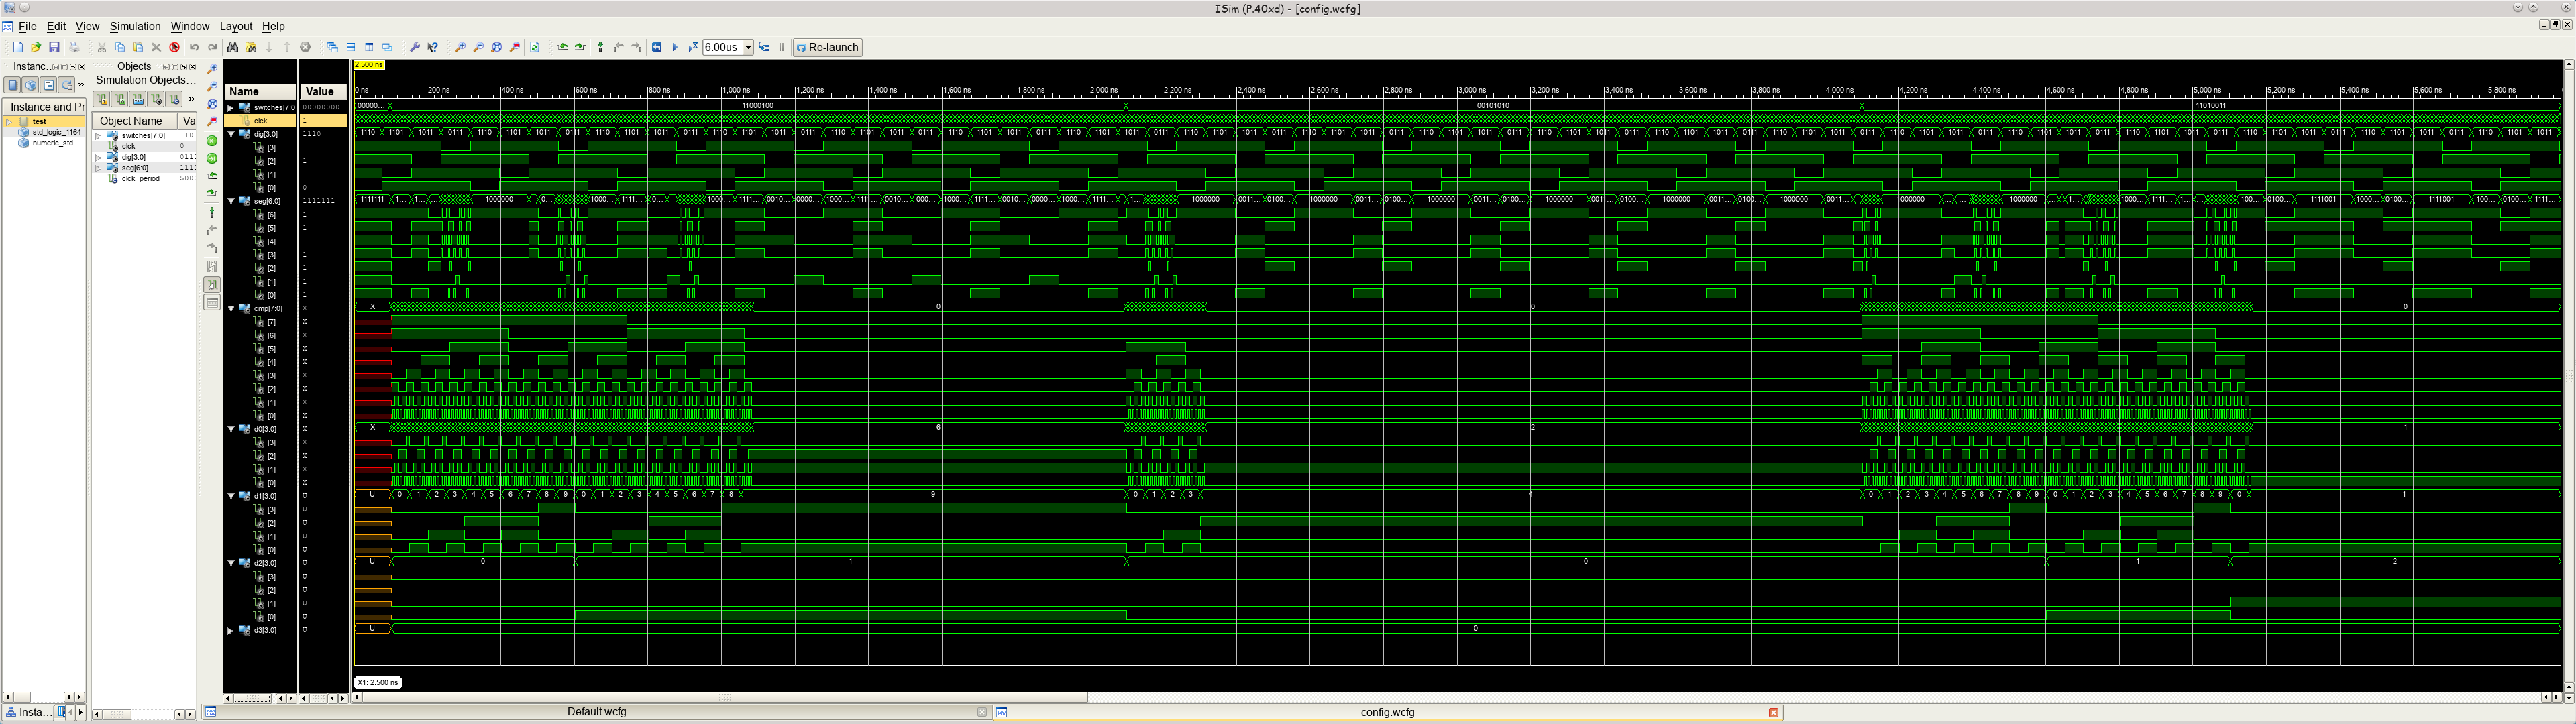
\includegraphics[scale=0.12]{Debug.png}
	\caption{View of the simulator}
\end{figure}

The simulation enables one to investigate the configuration behaviour in an almost interactive way that greatly simplifies the searching of errors. It gives a tracking in time and of the impedances through the whole circuit as they should be in a physical device.

The simulation is supported inside VHDL, with special statements (wait for 2ms, for example) or data types (floats) that are not supported by the synthesizer but that make the analysis easier.

The simulation configuration consist of a separated VHDL file that defines the inputs values through the simulation time.


\subsection{Existing high level compilers}

The complexity of VHDL and it's distance to usual software programming languages prevent programmers from using it.
To give an easier way to introduce hardware in software applications, some high-level compilers have been developed.

\subsubsection{Targeted execution environments}

Most of the high-level compilation tools targets highly heterogeneous systems, aiming at providing a unique language to describe both software and hardware parts. These execution environments can be composed of multiple CPUs, GPUs, FPGAs or other specific hardware devices.

These systems have in common the existence of a main processor (CPU) that will organised the compilation.

OpenCL...

\subsubsection{Xilinx's Vivado tool}

The Vivado Design Suite gathers tools to develop a software application with hardware parts. It gives a C to HDL compiler that enables to describe hardware parts in C.

The tool compiles each hardware source to an entity, inlining the called functions.

It adds a set of signals to each function that enable to link the different parts of the project (see section \ref{Opts} for details about it).
These signals are :
\begin{itemize}
	\item \textbf{Input start signal} : has to be activated when new entries are send to the input ports.
	\item \textbf{Output done signal} : tells that the computation is finished for the latest entries in computation.
	\item \textbf{Output idle signal} : tells if a computation is in process.
	\item \textbf{Output ready signal} : tells if new entries can be sent.
\end{itemize}

The C statements are compiled to their equivalent VHDL concurrent statements, and processes are used to update the additional signals.

Unbound loops are supported through the generation of a complex state machine.

\subsubsection{Limitation}

Several projects of high level compiler only compile a very small subset of the original language to its obvious equivalent, using a main VHDL process (C to VHDL).
These solutions only bridge the gap between the syntax (quiet a huge one) and leave to the programmer the understanding of how VHDL is actually compiled.


\section{The Whiley language and the compiler framework}

\subsection{The Whiley Language}

\subsection{The Whiley Intermediate Language (Wyil)}


\section{The WhileyToWHDL Compiler}

\subsection{Code structure conversion}

The global structure of the code is kept in a strait-forward manner :
\begin{itemize}
	\item Each Wyil file is converted to a unique VHDL source file
	\item Each function of a file is converted to an entity and a corresponding architecture
\end{itemize}


\subsection{Types compilation}

\subsubsection{Primitive types}

The Wyil primitive types are compiled in an obvious way as follows :

\begin{itemize}
	\item int $\longrightarrow$ signed(31 downto 0) [Temporary]
	\item bool $\longrightarrow$ boolean
	\item byte $\longrightarrow$ std\_logic\_vector(7 downto 0) 
\end{itemize}

\subsubsection{Complex types}

Other types are represented as a tree with primitive types as leaves.

\begin{itemize}
	\item \textbf{Record types} : The root of the type tree contains the fields of the record type as children.
	\item \textbf{Union types} :
\end{itemize}

\subsection{Functions compilation}

Functions are compiled using concurrent statements, and use process statements only for the introduction of registers. 

\subsubsection{Building the Control-Flow graph}

To ensure the use of a fine grained parallelism, the data control-flow graph of each function is build.

It is done at the signal level, which means that values of complex types are separated is they atomic components.

This graph is made of two types of nodes : 
\begin{itemize}
	\item \textbf{Operation nodes} : represents a operation
	\item \textbf{Label nodes} : represents the name of the data at the corresponding place in the source file.
\end{itemize}

\paragraph{Remark :} The use of label nodes is not needed for the data-flow graph (the identifiers could be associated with each arrow) but it makes the signal naming easier when producing VHDL code. \\


This graph can then be internally  optimised and modified (inlining).

A extra care has to be taken with the management of returns : whereas they can be placed anywhere in the source code (inside some if statement), they need to be gathered in a unique output signal in the hardware design.

\subsubsection{Building a pipeline}

\label{Opts}

The conversion of this graph to VHDL is only one half of the work to be done. In order to make the components be connected with others or with other computation devices, some invariant in the production of data have to be arbitrary chosen and guaranteed.

Several options are possible to make the whole system work :

\paragraph{Cycle number guarantee}
~\\
The easiest solution to connect different circuits is to provide the same time execution guarantee for each part of the configuration. 

To avoid a low clock frequency, the computation should be split into several part separated by registers. To do this, the data-flow graph has to be split to know with value are needed in several pipeline steps.


\paragraph{State signals}
~\\
A state machine can be set up for each parts of the project, with some signals telling if the entity can read new data or if new outputs are ready. This solution has the benefit to support unbound calculations (loops) but prevent every time guarantee and lead to a bigger configuration.



\subsection{Implementation details}

Using Java

Compilation construct as a pipeline (The result of a step is given to the next one)
 
 
 
 
 \bibliographystyle{alpha}
 \bibliography{References}

\end{document}